\documentclass[fleqn,usenatbib]{mnras}

% MNRAS is set in Times font. If you don't have this installed (most LaTeX
% installations will be fine) or prefer the old Computer Modern fonts, comment
% out the following line
%\usepackage{newtxtext,newtxmath}
\usepackage{times}
% Depending on your LaTeX fonts installation, you might get better results with one of these:
% \usepackage{mathptmx}
% \usepackage{txfonts}

% Use vector fonts, so it zooms properly in on-screen viewing software
% Don't change these lines unless you know what you are doing
\usepackage[T1]{fontenc}
\usepackage{ae,aecompl}


%%%%% AUTHORS - PLACE YOUR OWN PACKAGES HERE %%%%%
%\usepackage{epsf}
\usepackage{color}
\usepackage{graphicx}
\usepackage{amsmath}	% Advanced maths commands
\usepackage{amssymb}	% Extra maths symbols
\usepackage{mathrsfs}	% Extra extra math symbols
\usepackage{natbib}
%\usepackage[colorlinks,urlcolor=magenta,citecolor=blue,linkcolor=blue]{hyperref}
\usepackage{multirow}
\usepackage{etoolbox}
\usepackage{listings}

\graphicspath{{./figures/}}

%%%%% AUTHORS - PLACE YOUR OWN COMMANDS HERE %%%%%
%%% Fields %%%
\newcommand{\hdf}{HDF-N}
\newcommand{\hdfn}{HDF-N}
\newcommand{\hdfs}{HDF-S}
\newcommand{\cdfs}{CDF-S}

%%% Telescopes %%%
\newcommand{\hst}{\textit{HST}}
\newcommand{\iras}{\textit{IRAS}}
\newcommand{\iso}{\textit{ISO}}
\newcommand{\spitzer}{\textit{Spitzer}}
\newcommand{\sirtf}{\textit{Spitzer}}
\newcommand{\chandra}{\textit{Chandra}}

%%% Filters %%%
\newcommand{\wfu}{\hbox{$\mathrm{U}_{300}$}}
\newcommand{\wfb}{\hbox{$\mathrm{B}_{450}$}}
\newcommand{\wfv}{\hbox{$\mathrm{V}_{606}$}}
\newcommand{\wfi}{\hbox{$\mathrm{I}_{814}$}}
\newcommand{\acsb}{\hbox{$\mathrm{B}_{435}$}}
\newcommand{\acsv}{\hbox{$\mathrm{V}_{606}$}}
\newcommand{\acsi}{\hbox{$i_{775}$}}
\newcommand{\acsz}{\hbox{$z_{850}$}}
\newcommand{\nicj}{\hbox{$\mathrm{J}_{110}$}}
\newcommand{\nich}{\hbox{$\mathrm{H}_{160}$}}
\newcommand{\wfcy}{\hbox{$\mathrm{Y}_{105}$}}
\newcommand{\wfcj}{\hbox{$\mathrm{J}_{125}$}}
%\newcommand{\wfcj}{\hbox{$J_{110}$}}
\newcommand{\wfch}{\hbox{$\mathrm{H}_{160}$}}
\newcommand{\sdssu}{\hbox{$u$}}
\newcommand{\sdssg}{\hbox{$g$}}
\newcommand{\sdssr}{\hbox{$r$}}
\newcommand{\sdssi}{\hbox{$i$}}
\newcommand{\sdssz}{\hbox{$z$}}
\newcommand{\mone}{\hbox{$[3.6]$}}
\newcommand{\mtwo}{\hbox{$[4.5]$}}
\newcommand{\mthree}{\hbox{$[5.8]$}}
\newcommand{\mfour}{\hbox{$[8.0]$}}
%\newcommand{\mone}{\hbox{$[3.6\mu\mathrm{m}]$}}
%\newcommand{\mtwo}{\hbox{$[4.5\mu\mathrm{m}]$}}
%\newcommand{\mthree}{\hbox{$[5.8\mu\mathrm{m}]$}}
%\newcommand{\mfour}{\hbox{$[8.0\mu\mathrm{m}]$}}

%%% Astronomy Abreviations %%%
\newcommand{\mstar}{\hbox{$\mathrm{M}^\ast$}}
\newcommand{\lstar}{\hbox{$L^\ast$}}
\newcommand{\Msol}{\hbox{$\mathrm{M}_\odot$}}
\newcommand{\msol}{\hbox{$\mathrm{M}_\odot$}}
\newcommand{\Zsol}{\hbox{$Z_\odot$}}
\newcommand{\zsol}{\hbox{$Z_\odot$}}
\newcommand{\Lsol}{\hbox{$L_\odot$}}
\newcommand{\lsol}{\hbox{$L_\odot$}}
\newcommand{\lir}{\hbox{$L_{\mathrm{IR}}$}}
\newcommand{\zph}{\hbox{$z_\mathrm{ph}$}}
\newcommand{\zphot}{\hbox{$z_\mathrm{ph}$}}
\newcommand{\lbol}{\hbox{$L_\mathrm{bol}$}}
\newcommand{\snr}{\hbox{$\mathrm{S/N}$}}
\newcommand{\reff}{\hbox{$r_\mathrm{eff}$}}
\newcommand{\ks}{\hbox{$K_s$}}
\newcommand{\AAA}{\hbox{\AA}}

%%% Spectrum Lines %%%
\newcommand{\lya}{ Ly$\alpha \;$}
\newcommand{\lyb}{Lyman~$\beta$}
\newcommand{\hb}{\hbox{H$\beta$}}
\newcommand{\ha}{\hbox{H$\alpha$}}
\newcommand{\paa}{\hbox{Pa$\alpha$}}

%%% Units %%%
\newcommand{\kms}{\hbox{km~s$^{-1}$}}
\newcommand{\cms}{\hbox{cm~s$^{-1}$}}
\newcommand{\mpc}{\hbox{Mpc$^{-1}$}}
\newcommand{\mpcsq}{\hbox{Mpc$^{-2}$}}
\newcommand{\mpccu}{\hbox{Mpc$^{-3}$}}
\newcommand{\cnts}{\hbox{cnt~s$^{-1}$}} 
\newcommand{\cmsq}{\hbox{cm$^{-2}$}}
\newcommand{\cmcu}{\hbox{cm$^{-3}$}}
\newcommand{\ergscm}{\hbox{erg~s$^{-1}$~cm$^{-2}$}}
\newcommand{\uJy}{\hbox{$\mu$Jy}}
\newcommand{\ujy}{\hbox{$\mu$Jy}}
\newcommand{\degree}{\hbox{$^\circ$}}
\newcommand{\degsq}{\hbox{degree$^2$}}
\newcommand{\arcminsq}{\hbox{arcmin$^2$}}
\newcommand{\um}{\hbox{$\mu$m}}

%%% Math %%%
\newcommand{\lsim}{\lesssim}
\newcommand{\gsim}{\gtrsim}
\newcommand{\mathS}{\hbox{$\mathcal{S}$}}
\newcommand{\mathR}{\hbox{$\mathcal{R}$}}
\newcommand{\mathM}{\hbox{$\mathcal{M}$}}
\newcommand{\mcal}{\hbox{$\mathcal{M}$}}
\newcommand{\rcal}{\hbox{$\mathcal{R}$}}
\newcommand{\scal}{\hbox{$\mathcal{S}$}}
\newcommand{\infinity}{\hbox{$\infty$}}
\newcommand{\err}[2]{$^{+#2}_{-#1}$}

%%% General %%%
\newcommand{\etal}{et al.}
\newcommand{\eg}{e.g.}
\newcommand{\ie}{i.e.}
\newcommand{\cf}{cf.}
% \newcommand{\ion}[2]{\hbox{#1$\;${\small\rm{#2}}}}
\newcommand{\mybullet}{\noindent$\bullet$}
\newcommand{\uit}{\textit{UIT}}
\newcommand{\nd}{...}
%\newcommand{\cmodel}{\hbox{\tt cmodel}}
%\newcommand{\bs}{\hbox{$\!\!\!\!$}}
\newcommand{\todo}[1]{{\tt #1}}
\newcommand{\citeeg}[1]{(\eg, \citealt{#1})}
\newcommand{\ignore}[1]{}

%%% Extra %%% 
% \newcommand{\farcm}{\mbox{\ensuremath{.\mkern-4mu^\prime}}}%fractional arcminute symbol 0.'0
% \newcommand{\farcs}{\mbox{\ensuremath{.\!\!^{\prime\prime}}}}%fractional arcsecond symbol: 0.''0
% \newcommand{\fdg}{\mbox{\ensuremath{.\!\!^\circ}}}%fractional degree symbol:     0.°0
\newcommand{\arcdeg}{\ensuremath{^{\circ}}}%                    % degree symbol:  °
% \newcommand{\sun}{\ensuremath{\odot}}%                          % sun symbol
% \newcommand{\apj}{ApJ}%                                         % Journal abbreviations
% \newcommand{\apjs}{ApJS}
% \newcommand{\apjl}{ApJL}
% \newcommand{\aap}{A{\&}A}
% \newcommand{\aaps}{A{\&}AS}
% \newcommand{\mnras}{MNRAS}
% \newcommand{\aj}{AJ}
% \newcommand{\araa}{ARAA}
% \newcommand{\pasp}{PASP}
\newcommand{\Teff}{\ensuremath{T_{\mathrm{eff}}}}%              % T_eff
\newcommand{\logg}{\ensuremath{\log g}}%                        % log g
\newcommand{\bv}{\ensuremath{B\!-\!V}}%                         % B-V
\newcommand{\ub}{\ensuremath{U\!-\!B}}%                         % U-B
\newcommand{\vr}{\ensuremath{V\!-\!R}}%                         % V-R
\newcommand{\ur}{\ensuremath{U\!-\!R}}%                         % U-R

\newcommand{\editorial}[1]{\textcolor{red}{#1}}
\newcommand{\multic}[2]{\multicolumn{#1}{c}{#2}}
\newcommand{\rottext}[2]{\multirow{#1}{*}{\rotatebox[origin=c]{90}{#2}}}

%%%%%%%%%%%%%%%%%%% TITLE PAGE %%%%%%%%%%%%%%%%%%%
\title[Metallicity with CNNs]{Predicting Galaxy Metallicity from Three-Color Images using Convolutional Neural Networks}

% The list of authors, and the short list which is used in the headers.
% If you need two or more lines of authors, add an extra line using \newauthor
\author[Wu and Boada]
{\parbox{\textwidth}{John~Wu$^{1}$\thanks{E-mail: jw740@physics.rutgers.edu} and
Steven~Boada$^{1}$}\vspace{0.4cm}\
\\
\parbox{\textwidth}{$^{1}$Physics and Astronomy Department, Rutgers University, Piscataway, NJ 08854-8019, USA\\}}

% These dates will be filled out by the publisher
\date{Accepted XXX. Received YYY; in original form ZZZ}

% Enter the current year, for the copyright statements etc.
\pubyear{2018}

% Don't change these lines
\begin{document}
\label{firstpage}
\pagerange{\pageref{firstpage}--\pageref{lastpage}}
\maketitle

\begin{abstract}
\noindent
Lorem ipsum dolor sit amet, consectetur adipisicing elit, sed do eiusmod tempor incididunt ut labore et dolore magna aliqua. Ut enim ad minim veniam, quis nostrud exercitation ullamco laboris nisi ut aliquip ex ea commodo consequat. Duis aute irure dolor in reprehenderit in voluptate velit esse cillum dolore eu fugiat nulla pariatur. Excepteur sint occaecat cupidatat non proident, sunt in culpa qui officia deserunt mollit anim id est laborum.
\end{abstract}

\section{Introduction}\label{sec:introduction}
\editorial{Things we are going to want to talk about in the introduction: Morphology-metalicity relation? There is certainly a mass-metallicity relation. Basically, we want to say why we think we can do this at all? What is the primary science driver behind why we think this will work? Is it really just the fundamental plane? We aren't telling the thing about the mass or the distance to the objects.}


\editorial{Spectral super-resolution?}

Large-area sky surveys, both on-going and planned, are revolutionizing our understanding of galaxy evolution. The on going Dark Energy Survey (DES; \citealt{DES2005}) and planned Large Synoptic Survey Telescope (LSST; \citealt{LSST2012}) will survey vast swaths of the sky and create samples of galaxies much larger than any previously know. Spectroscopic follow-up will be key to a deep understanding of the properties of these galaxies, and constrain galaxy evolution (e.g., the mass-metallicity relation, \citealt{Tremonti+05}; or the fundamental metallicity relation, \citealt{2010paper,2011paper}). But as the dataset continues to grow individual follow-up becomes increasingly impractical. Therefore, large spectroscopic surveys are needed to more fully understand the observable-mass relation of clusters.
In this work, we propose to use supervised ML, specifically convolution neural networks, to analyze pseudo-three color images to predict galaxy metallicity.
This paper is organized as follows: Section \ref{sec:CNN} we briefly introduce convolutional neural networks, discuss selection of the network's hyperparameters and outline training the network. In Section~\ref{sec:data}, we describe the acquisition and cleaning of the SDSS data sample. We present the main results in Section~\ref{sec:results} and discuss the results in the context of previous works in Section~\ref{sec:discussion}. In Section~\ref{sec:summary}, we summarize the key results and conclude.
Unless otherwise noted, throughout this paper, we use a concordance cosmological model ($\Omega_\Lambda = 0.7$, $\Omega_m = 0.3$, and $H_0= 70$ \kms \mpc), assume a Chabrier initial mass function \citep{Chabrier2003}, and use AB magnitudes \citep{Oke1974}.

\section{Methodology} \label{sec:methodology}

\subsection{Convolutional neural networks}
In recent years, neural networks have been able to accomplish a large number of tasks in the field of machine learning (LeCun et al. 1989).
Image classification and regression problems are most readily solved by use of convolutions in mutliple layers of the network (see, e.g., Krizhevsky et al. 2012).
Convolution neural networks (CNNs, or convnets) efficiently learn spatial relations in images whose features are about the same sizes as the convolution filters (or kernels) which are to be learned through training.
CNNs are considered \textit{deep} when the number of convolutional layers is large; visualizing their filters reveals that increased depth permits the network to learn more and more abstract features (e.g., from Gabor filters, to geometric shapes, to faces; Zeiler \& Fergus 2013).

The input layer is simply an image of $128\times 128$ pixels with three channels (RGB).
Dieleman et al. (Galaxy Zoo Kaggle competition) have already shown that CNNs are capable of classifying the morphologies of such images of galaxies from the Sloan Digital Sky Survey (SDSS) with the same accuracy as citizen scientists.
Other people have been done other cools things (like use simulated images to select real galaxies, etc).
blah blah blah.
Define overfitting: a specific and usually not general set of features are learned and misapplied to the test set data.


\subsection{Training in practice} \label{sec:training}

We split our training sample of $\sim 130,000$ images into sets of $90,000$ for training, $20,000$ for validation, and $20,000$ for testing.
Training images are seen once every epoch, although usually each epoch is split into a number of mini-batches which are learned in parallel.
Mini-batches are usually small ($256?$) and potentially not representative of the full training sample -- another technique used to prevent overfitting.
Each mini-batch is fed forward through the input layers, where a random fraction of connections $p=0.25, 0.50$ are removed between each linear layer (dropout, Hinton et al. 2012; see subsection below).
When the feed-forward network reports a prediction, whether a single or set of quantities, then a loss/cost function is used to compute how incorrect the prediction ($\hat y$) is from the true value $y$.
We use the root mean squared error (RMSE$~\equiv \sqrt{\langle |\hat y - y|^2\rangle}$) loss function, and seek to minimize it.
We use gradient descent for each mini-batch to adjust each weight parameter, and each fractional contribution of loss is determined by the backpropagation algorithm (cite original, LeCun et al.).
The backpropagation algorithm is simply the chain rule applied to finite derivatives, and skipped? for any non-linear layers.
The gradient is multiplied by the \textit{learning rate}; batch-normalization is also applied in addition to a momentum term which ensures that the gradient is itself only changing slowly with each mini-batch.


CNNs become difficult to train after many layers are added, likely because the network has already found the best representation possible at a shallower layer, and further layers simply noisily propagate the same signal and degrade the loss.
We select an architecture called a residual neural network, or a \textit{resnet} (He et al. 2015), which contains enhanced ``shortcut connections'' but are otherwise similar to other CNNs.
Resnets have been shown to continue learning with increasing depth without the added cost of extra parameters.
%Therefore resnets are able to learn deep representations of the data.

We use a 34-layer resnet (He et al.), whose architecture consists of three layer groups.
Our resnet is initialized to pre-trained weights from the ImageNet data set, which consists of 1.7~million images belonging to 1000 categories of objects found on Earth (e.g., cats, horses, cars, or books).
The earlier layer groups generally have already trained filters that represent low-level abstractions, such as edges or Gabor filters, so we first train only the last layer group of the network (and ``freeze'' the weights in the first two groups).
By reducing the number of trainable parameters, we can rapidly approach the global loss minimum in a few number of epochs.
We train the final layers for two epochs using a learning rate of 0.1, and then ``unfreeze'' the earlier layers and train for another eight epochs using learning rates of [0.001, 0.01, 0.1] for the first, second, and third layer group respectively.
For more details about our training methodology, such as the use of learning rate annealing, data augmentation, dropout, batch-normalization, and other hyperparameters, see the Appendix.

Our training methods near convergence after 10 epochs, and additional training only marginally improves the loss.
In total, our training steps requires 25-30 minutes on our GPU and uses under 2~GB of memory (depending on batch size).
%Ensemble methods take $k$ times as long to train.
Prediction using data augmentation (see Appendix) takes two minutes for our full test set of 20,466 images, or approximately 6~milliseconds per image (or a little over 1~millisecond per image without augmentation).
%Super-convergent training the network takes about 10 hours on a GPU but only yield marginal improvements over the ensemble methods (RMSE~$= 0.0828$ for super-convergent versus $0.0835$ for 5-fold).


In comparison, Huertas-Company et al. 2015 train their network for 10 days on a GPU following the Galaxy Zoo architecture.


We evaluate predictions using not only the RMSE, which approaches the standard deviation for Gaussian-distributed data, but also the NMAD, or the normal median absolute deviation:
\begin{equation}
{\rm NMAD}(x) \approx 1.4826 \times {\rm median} \big (\big|x - {\rm median }(x) \big|\big ),
\end{equation}
where for a Gaussian-distributed $x$, the NMAD will also approximate the standard deviation, $\sigma$.
NMAD is insensitive to outliers for non-Gaussian distributions and is useful for comparing scatter.

Glossary of terminology:
\begin{itemize}
	\item $Z \equiv 12 + \log ({\rm O/H})$ is the nebular phase metallicity
	\item $Z_{\rm true}$ is the spectroscopically derived metallicity
	\item $Z_{\rm pred}$ is the CNN predicted metallicity
	\item $\Delta Z \equiv Z_{\rm pred} - Z_{\rm true}$ is the residual, or error
	\item RMSE~$\equiv \sqrt{\langle |\hat y - y|^2\rangle}$ is the root-mean squared error. 
	The RMSE loss function is minimized during CNN training.
	\item NMAD~$\approx 1.4826 \times {\rm median} \big (\big|x - {\rm median }(x) \big|\big )$ is the normal median absolute deviation
\end{itemize}


\section{Data} \label{sec:data}

\subsection{Sample selection}

Our sample of galaxies are selected from the NYU Value Added Catalog (VAC) \editorial{cite}, to have gas phase metallicities. The 50th percentile metallicity estimates \citep{Tremonti2004} are derived from spectroscopic measurements and for the purposes of this work are assumed to be ``the truth.'' In addition, we take the derived stellar mass for each galaxy.
We supplement the data from the VAC with data from SDSS Data Release 13 (DR13; \citealt{Albareti2017}) for each galaxy, the right ascension and declination and the magnitude in each of the five SDSS photometric bands (\sdssu, \sdssg, \sdssr, \sdssi, \sdssz), along with associated errors. We require that galaxies magnitudes are $10 < \sdssu\sdssg\sdssr\sdssi\sdssz < 25$ mag. Galaxies should have colors $0 < \sdssu-\sdssr < 6$ \editorial{why?}, high confidence ($z_{err} < 0.01$) spectroscopic redshifts greater than \editorial{$0.2$}, \editorial{check the petro mags and why we are using those}.

\subsection{SDSS Images}

From this input catalog we create RGB images with the SDSS cutout service\footnote{\url{http://skyserver.sdss.org/dr14/SkyserverWS/ImgCutout/getjpeg}}. Images are scaled to be $128\times128$ pixels in size, corresponding to $15''\times15''$ on the sky. The native $0\farcs396$ SDSS pixel size are rescaled to $0\farcs296$ per pixel.
We obtain $142,176$ three color images to use as the full data set.
We split this data set into random 60\%, 20\%, and 20\% subsets, which comprise the training, validation, and test data sets respectively.

\subsection{Metallicity}


\section{Results}\label{sec:results}


\subsection{Example predictions}


\begin{figure*}
	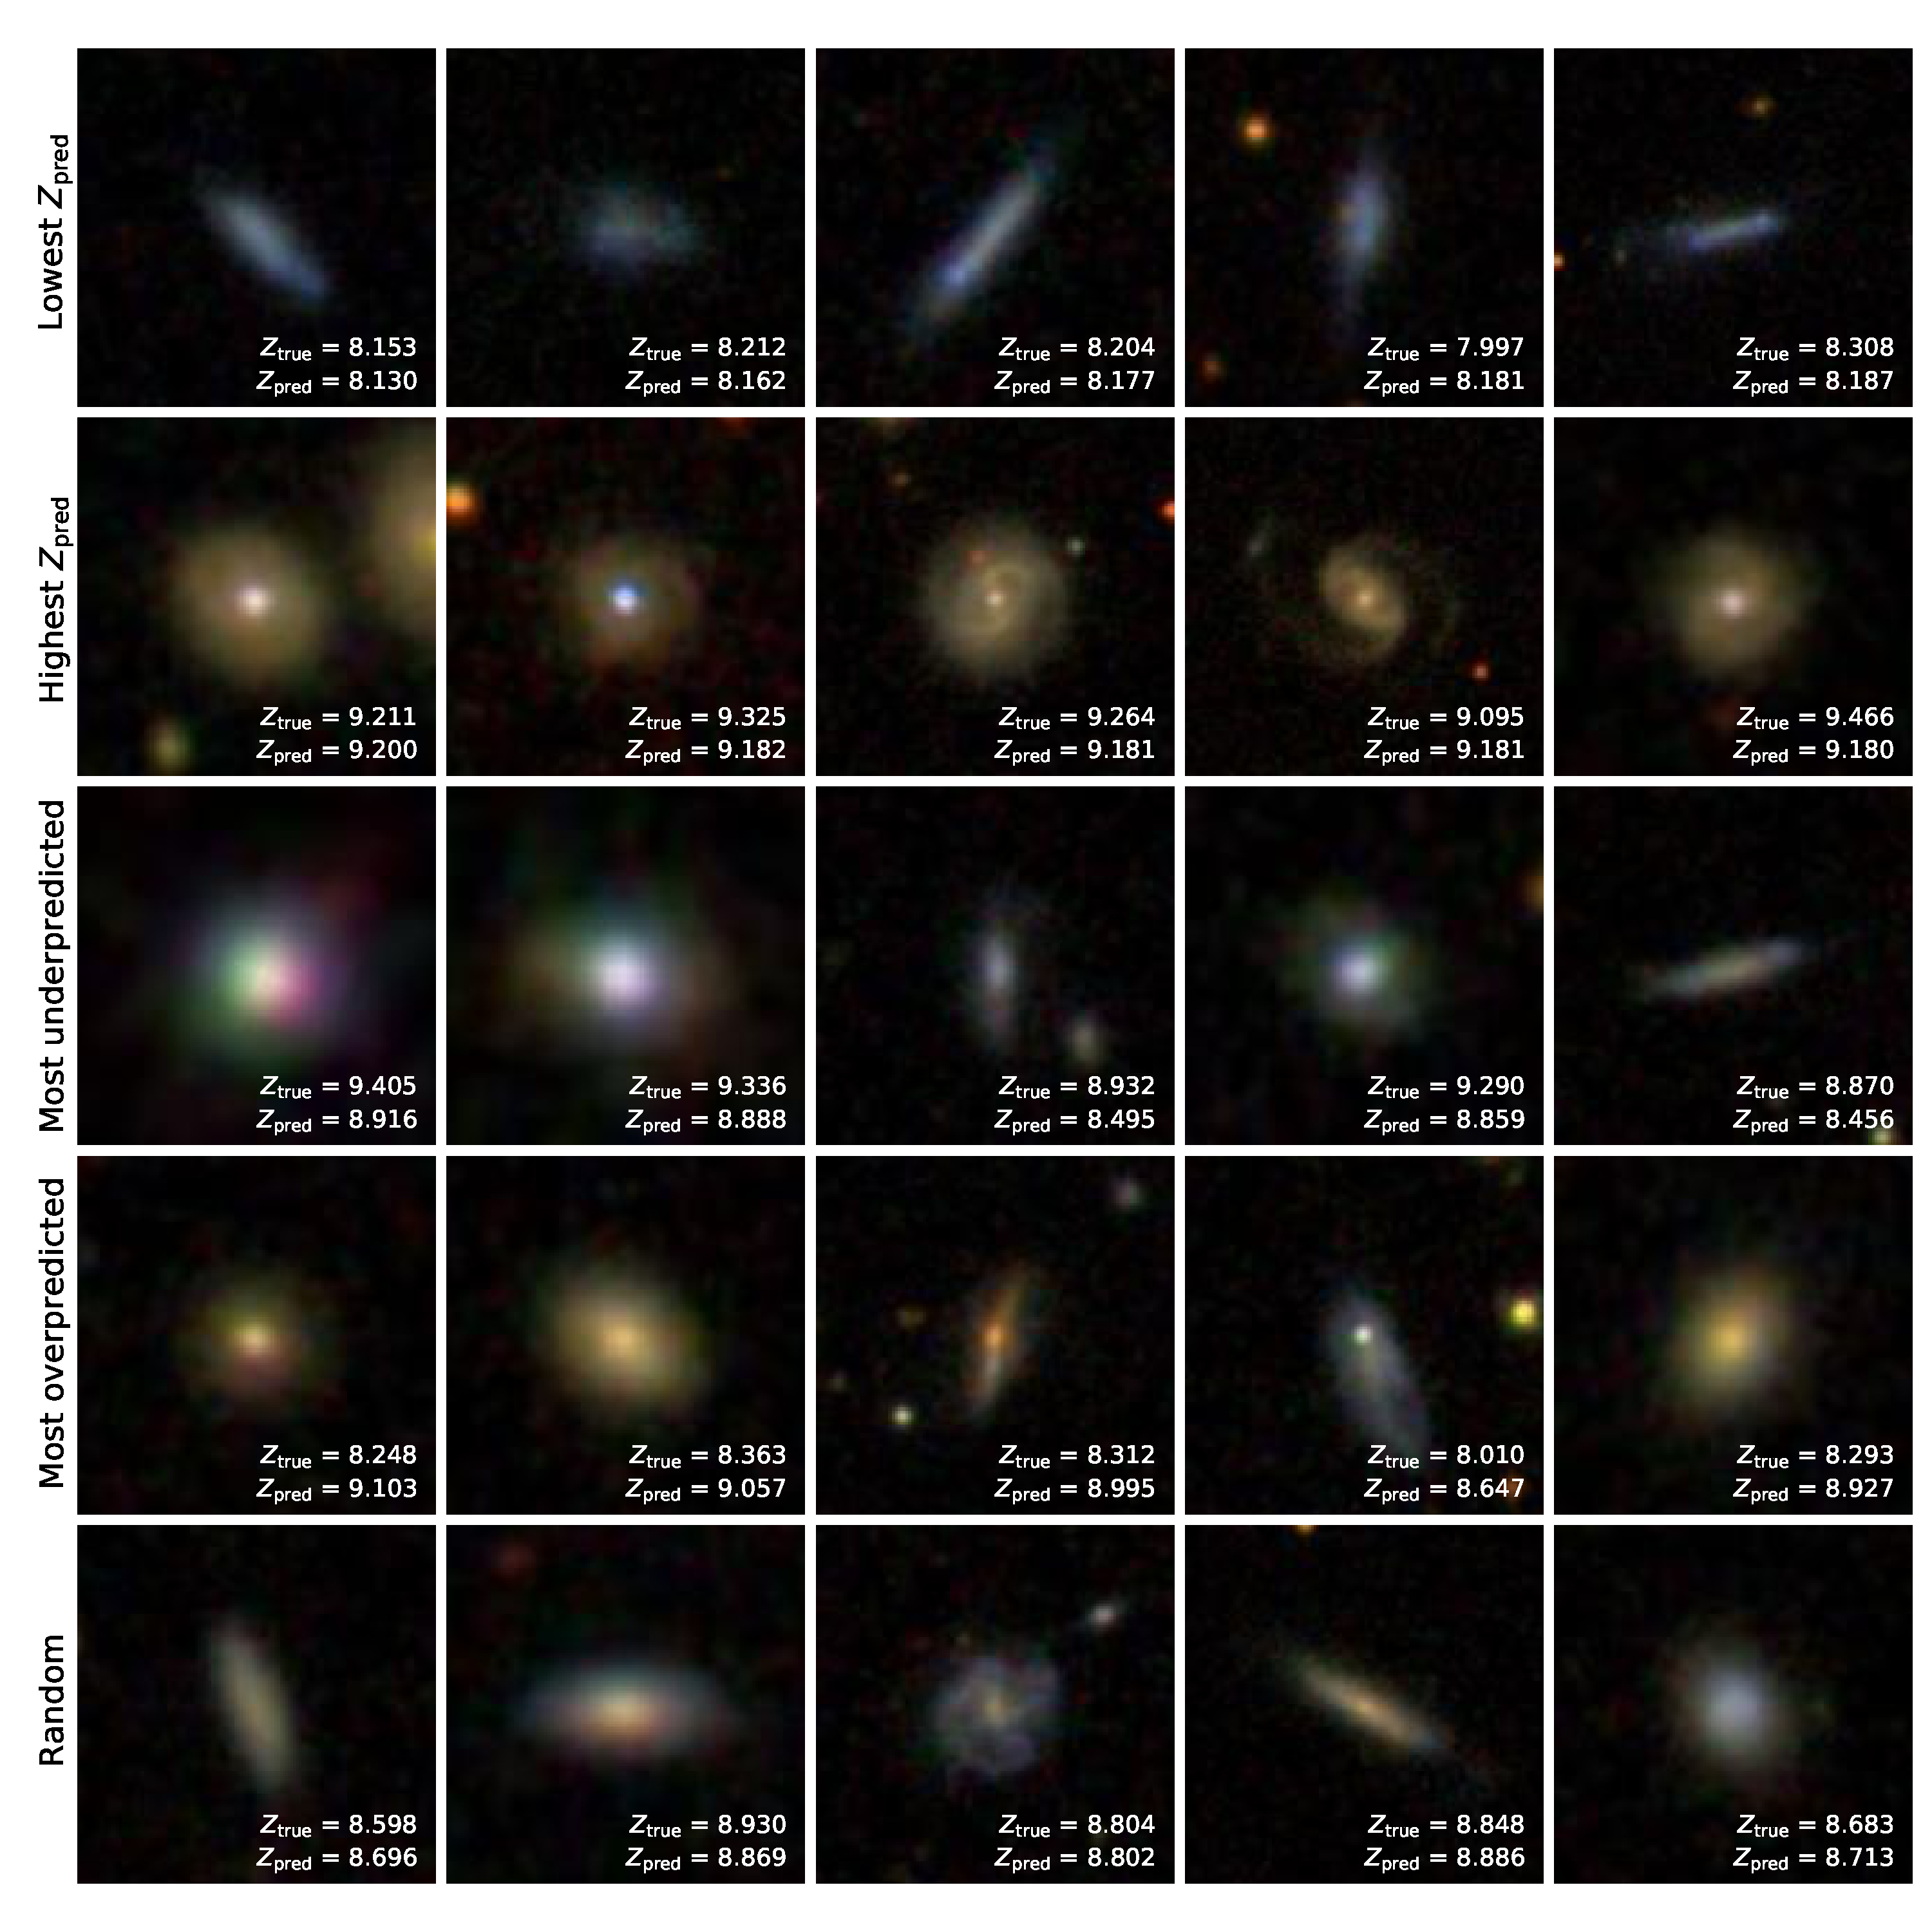
\includegraphics[width=0.9\textwidth]{01-prediction_examples.pdf}
	\caption{\label{fig:examples}
		SDSS imaging with predicted and true metallicities from the test data set. 
		Five examples are shown from each of the following categories: (a) lowest predicted metallicity, (b) lowest true metallicity, (c) highest predicted metallicity, (d) highest true metallicity, (e) most negative $\Delta Z \equiv Z_{\rm pred} - Z_{\rm true}$, (f) most positive $\Delta Z$, and (g) randomly selected galaxies.}
\end{figure*}


Examples of the $128 \times 128$ pixel $gri$ SDSS images fed into the the CNN are shown in Figure~\ref{fig:examples}.
Rows (a) and (b) depict the galaxies with lowest predicted and lowest true metallicities, respectively.
The CNN has associated blue, disky galaxies with low metallicities, and is generally accurate for those which it has identified to be low $Z_{\rm pred}$.
In rows (c) and (d), we show the galaxies with highest predicted and highest true metallicities, respectively.
Here we find that red galaxies containing prominent bulges or bright nuclei are predicted to be high in metallicity, and their predictions generally match $Z_{\rm true}$.
The main result appears to be that galaxies predicted by our CNN to have high metallicity ($Z_{\rm pred} > 9.0$) tend to truly have high metallicity, and the equivalent for low-metallicity galaxies.
Inversely, galaxies with the \textit{highest} or \textit{lowest} $Z_{\rm true}$ in the sample usually also yield high or low respective predicted metallicities.
Note that inclined galaxies tend to be lower in metallicity whereas face-on galaxies appear to be higher in metallicity.
\cite{2004ApJ...613..898T} explain this correlation by suggesting that the SDSS fiber aperture captures more column of a projected edge-on disk, allowing the metal-poor outer regions to depress the metallicity.

We will now consider examples of the most incorrectly predicted galaxies.
In rows (e) and (f) respectively, we show instances in which the CNN predicted too low metallicity and too high metallicity.
The two galaxies with lowest residuals $\Delta Z \equiv Z_{\rm pred} - Z_{\rm true}$ (i.e., most underpredicted metallicities) suffer from artifacts which cause unphysical color gradients.\footnote{Note that both are labeled as quasars according to their SDSS DR14 spectra. \editorial{A. Baker mentioned that it is possible some of the incorrect predictions in Figure~1 may be due to the fact that the $R_{23}$ estimator is a double-valued function, and the particular branch chosen may cause incorrect estimation of $Z_{\rm true}$. Such an effect may be possible if, e.g., one of the oxygen lines is at low SNR and the uncertainties are large.}}
Otherwise, the mistakes made by the CNN are similar to ones that human intuition are prone to make: blue, disky sources are generally thought of as lower in metallicity, and redder, more spheroidal objects tend to be higher in metallicity.

In the bottom row (g) of Figure~\ref{fig:examples}, we show five randomly selected galaxies.
The random SDSS assortment consists of elliptical, spiral, and possibly even an interacting pair of galaxies.
Residuals are low (below 0.15~dex), and we again find that the CNN predictions follow human visual intuition.


\subsection{Comparing predicted and true metallicities}

In Figure~\ref{fig:distributions}, we show the distributions of true and predicted metallicities.
The histogram bin sizes were chosen according to the \cite{Freedman1981} rule for each distribution.
The discreet striping of the Tremonti et al. and Brinchmann et al. metallicity estimator appears in the $Z_{\rm true}$ distribution (shown in black) but does not manifest in our CNN predictions (shown in red).
Because the true metallicities are discreetly valued, we expect that our distribution of $\Delta Z$ will be heavy-tailed, since predicted values still be distributed smoothly over the peaks and troughs in the $Z_{\rm true}$ distribution.
We also expect some outlier predictions at very negative or positive $\Delta Z$ for other reasons.

As we have described previously, the range of $Z_{\rm pred}$ is more limited than the range of $Z_{\rm true}$.
Too narrow a domain in $Z_{\rm pred}$ will lead to systematic errors, as the CNN will never predict very high or very low metallicities.
Although the two distributions are qualitatively consistent with each other at low metallicities (e.g., $Z < 8.5$).
However, the fraction of galaxies with high $Z_{\rm true} > 9.1$ ($2573/20466 = 12.6\%$) is more abundant than the fraction with high $Z_{\rm pred} > 9.1$ ($1174/20466 = 5.7\%$).
%However, $Z_{\rm true} > 9.1$ makes  of the test data set, whereas for only $1174/20466 = 5.7\%$ of predictions exceed $9.1$, so this discrepancy will lead to a shift toward negative residuals.


\begin{figure}
	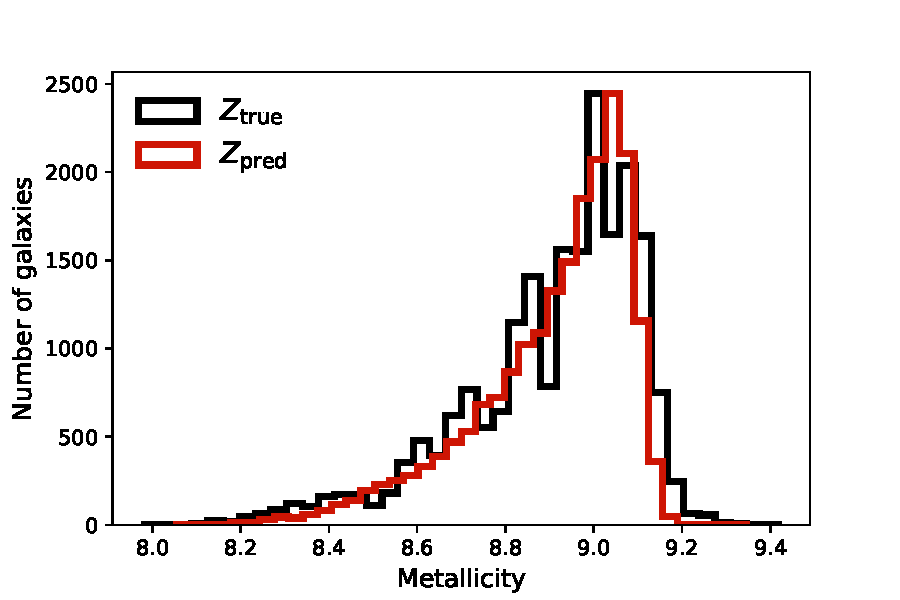
\includegraphics[width=\columnwidth]{03-Z_distribution.pdf}
	\caption{\label{fig:distributions}
		Distributions of the true (black) and predicted (red) galaxy metallicities.
		A distribution of residuals is shown in the inset panel.
		Note that the bin widths are different for each distribution.}
\end{figure}

\subsection{Scatter in $Z_{\rm pred}$ and $Z_{\rm true}$}


In Figure~\ref{fig:predicting-metallicity}, we compare the distributions of $Z_{\rm true}$ and $Z_{\rm pred}$ using a two-dimensional histogram (shown in grayscale in the main, larger panel).
We also show the median predictions varying with binned $Z_{\rm true}$ (solid red line), along with the scatter in RMSE (dashed blue) and NMAD (dashed orange), and also the one-to-one line (solid black).
Overall, the running median agrees well with the one-to-one line, although at low metallicity we find that the CNN makes makes overpredictions.
Thus, even though $Z_{\rm pred}$ and $Z_{\rm true}$ are in agreement at $Z < 8.5$ in Figure~\ref{fig:distributions}, we now find that the low-metallicity predictions are systematically too high.

A histogram of metallicity residuals is shown in the inset plot of the Figure~\ref{fig:predicting-metallicity} main panel.
The $\Delta Z$ distribution is characterized by an approximately normal distribution with a heavy tail at large positive residuals; this heavy tail is likely due to the systematic overprediction of low-$Z_{\rm true}$ galaxies.
%The median value of the distribution is $-0.006$, and a best-fit Gaussian function yields a centroid at $-0.009$.

We now turn our attention to the upper panel of Figure~\ref{fig:predicting-metallicity}, which shows how the scatter varies with spectroscopically derived metallicity.
The RMSE scatter and outlier-insensitive NMAD are both shown.
Marker sizes are proportional in area to the number of samples in each $Z_{\rm true}$ bin, and the horizontal lines are located at the average loss (RMSE or NMAD) for the full test data set.

Predictions appear to be both accurate and low in scatter for galaxies with $Z_{\rm true} \approx 9.0$, which is representative of an average metallicity in the SDSS sample.
Where the predictions are systematically incorrect, we find that the RMSE increases dramatically.
However, the same is not true for the NMAD: at $Z_{\rm true} < 8.5$, it asymptotes to $\sim 0.10$, even though the running median is incorrect by approximately the same amount!
This is because the MAD determines the scatter about the \textit{median} and not $\Delta Z = 0$, and thus, this metric becomes somewhat unreliable when the binned samples do not have a median value close to zero.
Fortunately, the global median of $\Delta Z$ is $-0.006$, or less than 10\% of the RMSE, and thus the global NMAD = 0.0668 is representative of the outlier-insensitive scatter for the entire test data set.

This effect partly explains why the global NMAD (0.0668) is higher than the weighted average of the binned NMAD ($\sim 0.05$).
Another reason why the global NMAD exceeds the binned NMAD average is that each binned NMAD is computed using its local scatter, and this allows for outlier rejection using a standard which varies with $Z_{\rm true}$.
We can demonstrate this result using an example: $\Delta Z \approx 0.2$ would be treated as an $3~\sigma$ outlier at $Z_{\rm true} = 9.0$, where the CNN is generally accurate, but the same residual would not be rejected as an outlier using NMAD for $Z_{\rm true} = 8.5$.
Since the binned average NMAD depends on choice of bin size, we do not include those results in our analysis and only focus on the global NMAD.

\begin{figure}
	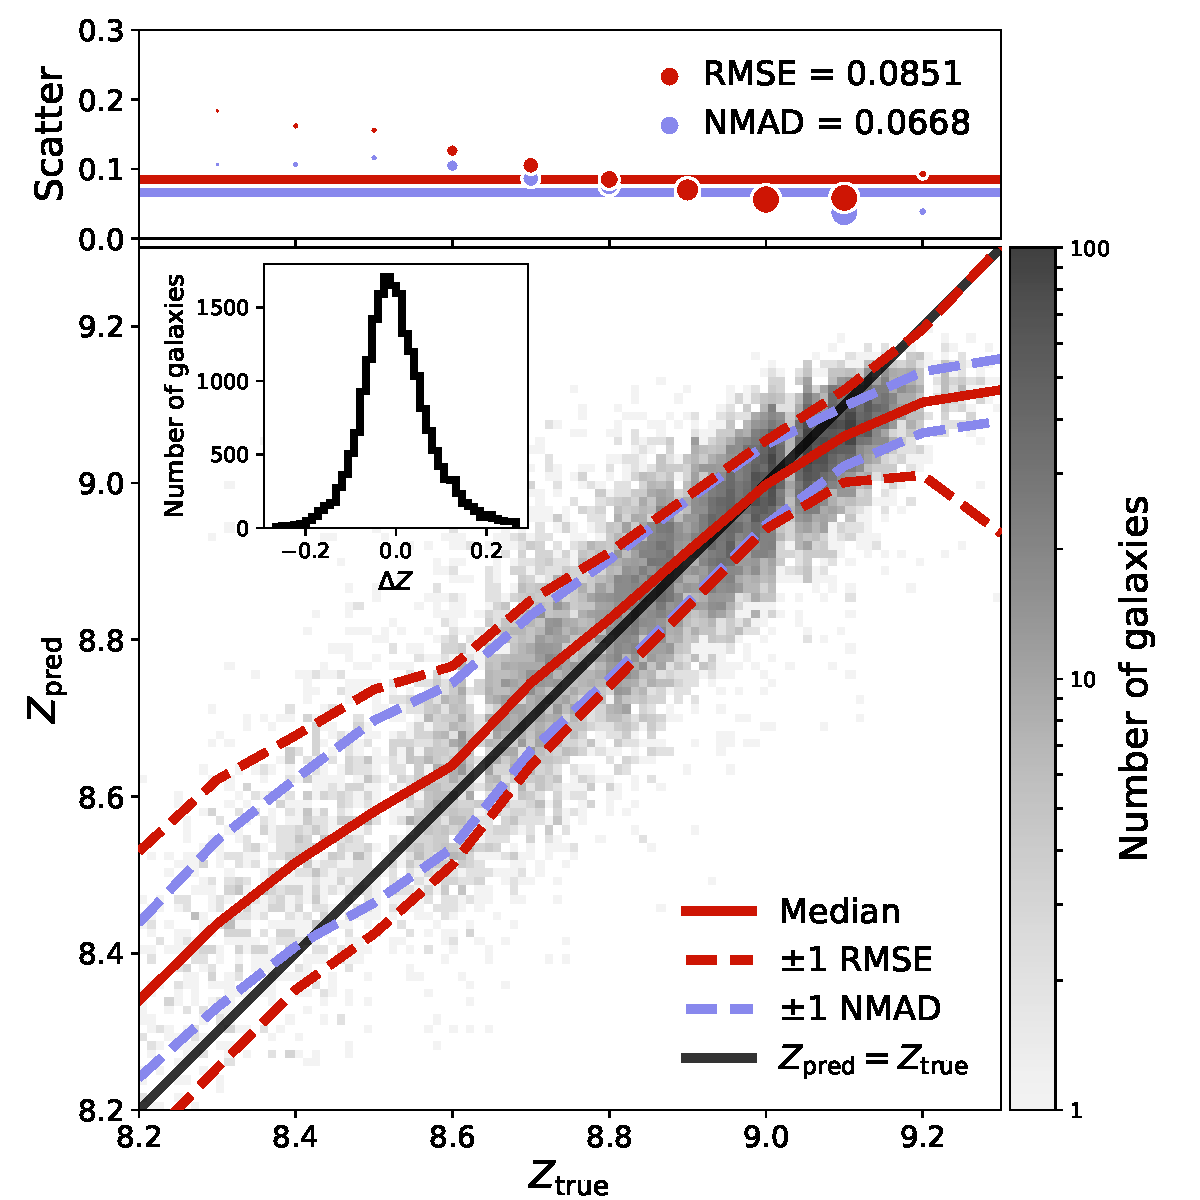
\includegraphics[width=\columnwidth]{02-prediction_summary.pdf}
	\caption{\label{fig:predicting-metallicity}
		Bivariate distribution of metallicity truths ($Z_{\rm true}$) and CNN predictions ($Z_{\rm pred}$) are shown in the main panel.
		Overlaid are the predicted median metallicity (\textit{solid red line}), RMSE scatter (\textit{dashed blue line}), NMAD scatter (\textit{dashed orange line}) in bins of $Z_{\rm true}$, and a one-to-one relation (\textit{solid black line}).
		In the upper panel, we again show the binned scatter, where the size of each marker is proportional to the number of galaxies in that bin.
		Each horizontal line corresponds to the average scatter over the entire test data set (and global value indicated in the upper panel legend).
		}
\end{figure}




\subsection{Resolution effects} \label{sec:resolution}

%Note by the way that our CNN trained on color images is able to predict better than by using only photometry (via random forest) and morphology ($r$-band CNN) independently.
%Perhaps this is due to the fact that morphology is correlated with stellar population age or something else.
%Color tells us the fundamental plane of SFR-$M_*$-metallicity but is biased by age and dust.


\begin{figure}
	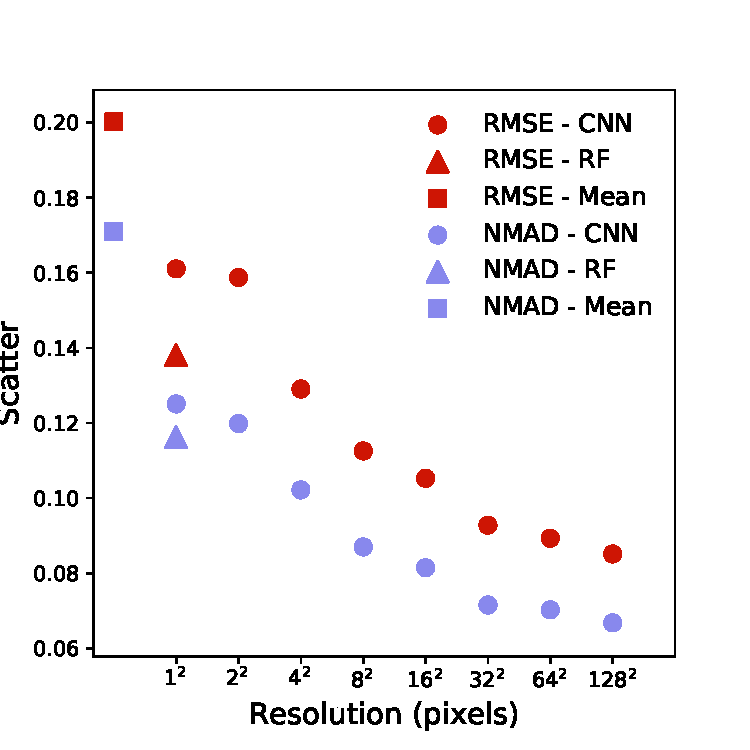
\includegraphics[width=\columnwidth]{04-resolution.pdf}
	\caption{\label{fig:resolution}
		The effects of image resolution on CNN performance.
		Blue and orange circular markers indicate scatter in the residual distribution ($\Delta Z$) measured using RMSE and NMAD, respectively.
		(Each point is analogous to the horizontal lines shown in Figure~\ref{fig:predicting-metallicity}.)
		We also show predictions from a random forest algorithm as stars-shaped markers, and constant $\langle Z_{\rm true}\rangle$ predictions as square markers.
	}
\end{figure}

Because our methodology is so computationally light, we can consider the effects of image resolution by running the exact same CNN training and test procedure on the same images scaled to different sizes.
Our initial results use SDSS $15\arcsec \times \arcsec$ cutouts resized to $128\times 128$ pixels, and we now downsample the images to $64\times 64$, $32 \times 32$, $\cdots$, $2\times 2$, and even $1\times 1$ pixels.
All images retain their three channels, so the smallest $1 \times 1$ image effectively contains three colors of the image (averaged together with its background and possible neighboring sources).


In Figure~\ref{fig:resolution}, we show the effects of image resolution by measuring the global scatter in $\Delta Z$ using the RMSE and NMAD metrics (shown in blue and orange circular markers, respectively).
Also shown is the scatter in $\Delta Z$ if we always predict the mean value of $Z_{\rm true}$ over the data set (shown using a square marker, and labeled ``Mean'').
This constant prediction is effectively the worst-possible scatter, and the SDSS systematic uncertainty in $Z_{\rm true}$ of $\sim 0.03$~dex is the best-possible scatter.
%In nearly all cases, we find that the NMAD is lower than the RMSE by a factor of $\sim 3/4$.
We find that both RMSE and NMAD decrease with increasing resolution.
The scatter is a strong function of resolution as the images are resolved from $2 \times 2$ to about $32 \times 32$.
With further increasing resolution, improvement is still evident, although the scaling with scatter is noticeably weaker.


There appears to be little improvement in scatter going from $1 \times 1$ to $2\times 2$ pixel images, although in hindsight such a finding should not be a surprise.
$1\times 1$ three-color images contain similar information to three photometric data points (although because of the averaged background and neighboring pixels, it is less useful than photometry), and three photometric data points can be used to perform a crude spectral energy distribution (SED) fit.
The color information is useful enough to create an approximate color-magnitude diagram, and each galaxy's position in this parameter space correlates with $Z_{\rm true}$.
The $2 \times 2$ three-color images contain four times as many pixels as the $1\times 1$ images.
However, because there is an even number of pixels, this information is still averaged between all available pixels, as so the incremental gain is small!\footnote{There is extra information in the $2\times 2$ pixel images in non-circularly symmetric cases. For an inclined disk, it is possible to roughly determine the orientation in the sky plane, but this information is not very useful. In the case of a major merger or interacting companion, the $2\times 2$ images may be more powerful than $1 \times 1$ images.}

\subsection{Random forest predictions}
We also construct a random forest (RF) of decision trees in order to predict metallicity, using the implementation from \texttt{scikit-learn} (cite).
Hyperparameters are selected according to the optimal RF trained by \cite{2016MNRAS.456.1618A}.
We use exactly the same data labels (i.e., galaxies) to train/validate or test the RF as we had done for training and testing the CNN, so that our measurements of scatter can be directly compared.
However, we have used the $gri$ three-band photometry data (given in magnitudes) to train and predict metallicity.
Since each galaxy only has three pieces of photometric information, it can be compared to the $1 \times 1$ three-band ``images'' processed by our CNN.


We note that the RF outperforms the CNN results using $1\times 1$ and $2 \times 2$ images.
This result is expected, given that the RF is supplied aperture-corrected photometry, whereas the CNN is given $1 \times 1 $ $gri$ ``images'' whose features have been averaged with their backgrounds.
$2 \times 2$ images are only marginally more informative.
When the resolution is further increased to $4 \times 4$ images, then the CNN can begin to learn rough morphological features and color gradients, which is already enough to surpass the performance (measured by both RMSE and NMAD) of the RF.

\subsection{Comparisons to Previous Works}\label{sec:previous work}

CNNs have been used for a wide variety of classification tasks in extragalactic astronomy, including morphological classification \citep[see, e.g.,][]{2015MNRAS.450.1441D,2015ApJS..221....8H,2017MNRAS.464.4420S}, distinguishing between compact and extended objects \citep{2017MNRAS.464.4463K}, selecting observational samples of rare objects based on simulations \citep{2018ApJ...858..114H,2018MNRAS.473.3895L}, and visualizing high-level morphological galaxy features \citep{2018arXiv180705657D}.
% Ellison group? 2016MNRAS.455..370E, 2017MNRAS.464.3796T, 2016MNRAS.457.2086T
% also 2018MNRAS.476.5516B?
These works seek to improve classification of objects into a discreet number of classes, e.g., visual morphologies.
Our paper uses CNNs to tackle the different problem of regression, i.e., predict values from a continuous distribution.

We have also found examples of regressing stellar properties in the astronomical machine learning literature \citep[see, e.g.,][]{2000A&A...357..197B,2018MNRAS.475.2978F}; they train on synthetic spectra and test on real data.
However, their true values of, e.g., stellar effective temperature, surface gravity, or elemental abundance, are known to be encapsulated in the synthetic stellar spectra.
Our work is novel because we predict metallicity, a spectroscopically determined galaxy property, only using three-color images --- and public-facing JPG images at that.
We have found that galaxy morphologies and colors contain information useful for predicting metallicity.


\cite{2016MNRAS.456.1618A} have used a variety of machine learning methods including RFs, extremely random trees (ERTs), boosted decision trees (AdaBoost), and support vector machines (SVMs) in order to estimate galaxy metallicity.
The data set used in this work consisted of a $z \sim 0.1$ sample (with $\sim 25,000$ objects) and a $z \sim 0.2$ sample (with $\sim 3,000$ objects), each of which had five-band SDSS photometry ($ugriz$) available as features.
These samples are sparsely populated at low metallicities, and they contain a smaller fraction of objects with $Z_{\rm true} < 8.5$ than our sample, but are otherwise similarly distributed in $Z_{\rm true}$ to ours.

We will first compare RF results, since this technique is common to both of our analyses, and reveals important differences in our training data.
Because outliers are defined differently in both works, we will use the RMSE metric to compare scatter between the two.
\cite{2016MNRAS.456.1618A} obtained RMSE of 0.081 and 0.093 when using RFs on the five-band photometry.
Using the same approach on a larger, unified, and different data set, which --- most importantly --- only contains \textit{three} bands of photometric information, we find RMSE = 0.1296.
Our scatter is larger than the value reported by \cite{2016MNRAS.456.1618A} by a factor of $\sim 150\%$.
This result may partly be explained by the fact that the $Z_{\rm true}$ distribution is narrower than for our data set, or the fact that we do not control for galaxy redshift; however, some of this advantage is offset by our larger sample size.
Ultimately, it appears the extra $u$ and $z$ bands provide valuable information, which allows for better estimation of metallicity.
RFs using the added photometry data output $Z_{\rm pred}$ with significantly lower scatter than our using only $gri$ bands.

Indeed, the $u$ and $z$ bands convey information about the star formation rate (SFR) and stellar mass ($M_\star$).
For this reason, it is possible that the RF trained on five-band photometry can estimate $Z_{\rm true}$ down to the limit of the FMR, which has very small scatter ($\sim 0.05$ dex) at given $M_{\star}$ \textit{and} SFR.
The $g$, $r$, and $i$ bands are rather insensitive to the SFR, but can still provide some information about the stellar mass, and so its results are more linked to the MZR rather than the FMR.



\section{The mass-metallicity relation} \label{sec:MMR}

The mass-metallicity relation (MZR) describes the tight correlation between galaxy stellar mass and nebular metallicity.
Scatter in this correlation is approximately $\sigma \approx 0.10$~dex in $Z_{\rm true}$ over the mass range $8.5 < \log (M_\ast / M_\odot) < 11.5$ \citep{2004ApJ...613..898T}, where $\sigma$ is the standard deviation of the metallicity and is equal to the RMSE for a normal distribution.
They characterize the MZR using a polynomial fit:
\begin{equation}\label{eq:mzr}
Z = -1.492 + 1.847 \log (M_\ast / M_\odot) - 0.08026 \left [\log(M_\ast / M_\odot)\right ]^2.
\end{equation}

The physical interpretation of the MZR is that a galaxy's mass strongly influences its chemical enrichment.
The origin of such a relationship is not clear, and proposed explanations include metal loss through blowout \citep[e.g.,][]{2002ApJ...581.1019G,2004ApJ...613..898T} inflow of pristine gas, or a combination of the two \citep[][]{2013ApJ...772..119L}; however, see also \cite{2013A&A...554A..58S}.
Although the exact physical process responsible for tight, $0.10$~dex scatter in the MZR is not known, its link to SFR via the FMR is clear, as star formation leads to both metal enrichment of the ISM and stellar mass assembly.
The FMR connects the instantaneous ($\sim 10$ Myr) SFR with the gas-phase metallicity \citep[$\sim 1$~Gyr timescales; see, e.g.,][]{2011ApJ...734...48L} and $M_{\ast}$ (i.e., the $\sim 13$~Gyr integrated SFR).
Our CNN is better suited for predicting $M_{\ast}$ rather than SFR, using the $gri$ bands, which can only weakly probe the bluer light from young, massive stars.
Therefore, we expect scatter from CNN predictions to be limited by the MZR (with scatter $\sigma \sim 0.10$~dex) rather than the FMR ($\sigma \sim 0.05$~dex).
It is possible that the color and morphology, in tandem with CNN-predicted stellar mass, can be used to roughly estimate the SFR, although any such relationship is not within the scope of our paper.



%Given the low scatter in metallicity residuals (predicted $-$ true), we consider if the CNN is able to accurately predict stellar mass, and then leverage the mass-metallicity relation (MMR; Tremonti et al. 2004) to infer metallicity.
%Alternatively, if SFR and $M_*$ are learned, then the fundamental metallicity relation (FMR; Mannucci et al. 2010, Lara-Lopez et al. 2010) may explain low residuals.


\subsection{Predicting stellar mass}

\begin{figure*}
	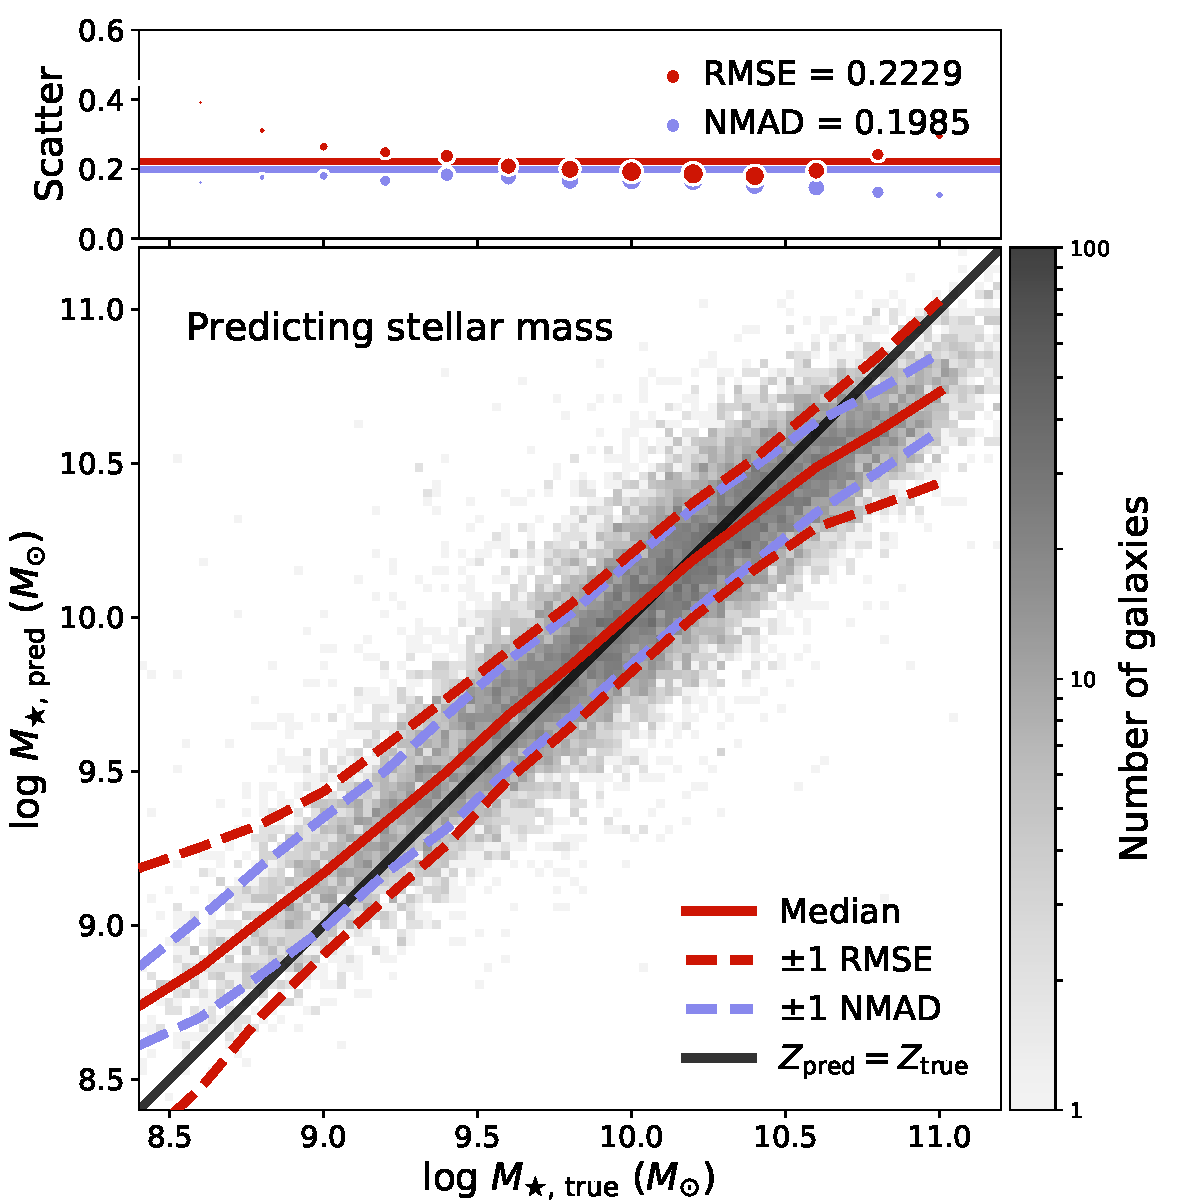
\includegraphics[width=\columnwidth]{05-a-prediction_mass.pdf}
	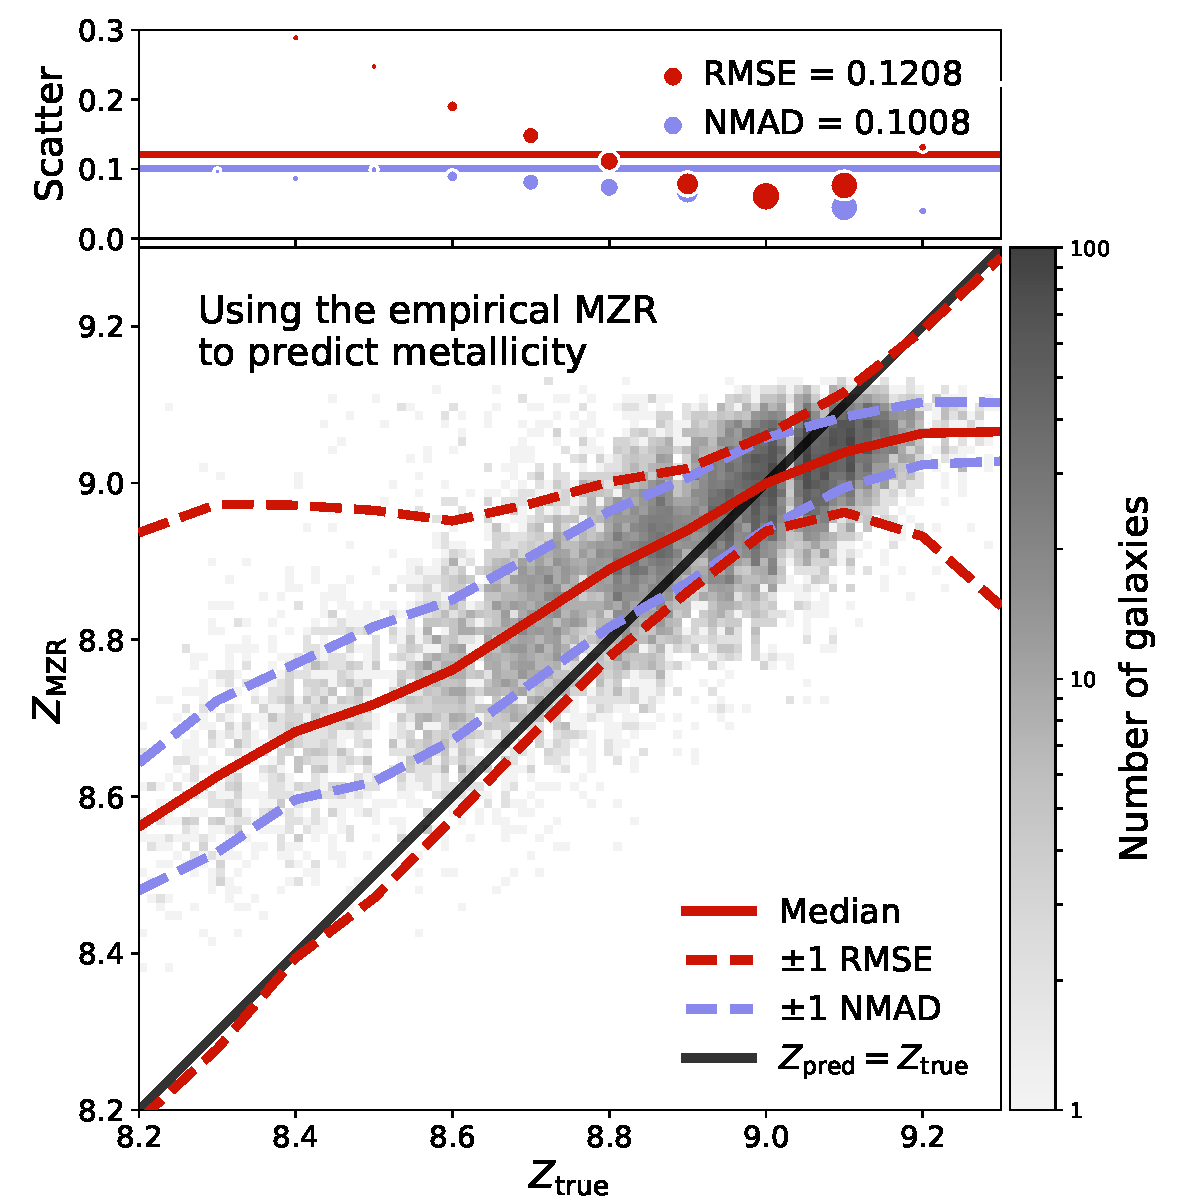
\includegraphics[width=\columnwidth]{05-b-prediction_mzr.pdf}
	\caption{\label{fig:mass-metallicity}
		In the left subplot, we show predicted against true stellar mass. 
		Colors and marker or line styles are the same as in Figure~\ref{fig:predicting-metallicity}.
		If the right subplot, we compare the predicted stellar mass converted to metallicity, assuming the Tremonti et al. mass-metallicity relation (MZR), with the true metallicity.}
\end{figure*}

We re-run the CNN methodology to train and predict $M_{\ast}$ using the 142,145 galaxies out of the original 142,186 that have available stellar mass measurements.
These results are shown in the left panel of Figure~\ref{fig:mass-metallicity}.
From the same subsample as before (minus three which do not have $M_{\ast}$), we verify that $M_{\rm \ast, true}$ median agrees with the median of $M_{\rm \ast, true}$ for values between $9.0 \lesssim \log M_\ast \lesssim 10.5$. 
The RMSE scatter in the $M_{\ast}$ residuals is $\sim 0.22$~dex, and the NMAD is $\sim 0.20$~dex.
The slope of the empirical MZR at $\log (M_\ast / M_\odot) \sim 10$ is (0.4~dex in $Z$)/(1.0~dex in $M_{\ast}$), implying that the CNN might be able to leverage the MZR and predict metallicity to $\sim 0.08$~dex (plus any intrinsic scatter in the MZR, in quadrature).
Given our CNN's ability to accurately predict $M_{\ast}$, coupled with the inability of SDSS images to inform it about nebular regions or spectral lines, is it possible that the CNN's unexpectedly strong performance in predicting metallicity comes through the MZR?

One option is that the CNN learned to predict $M_{\ast}$ followed by the polynomial MZR transformation (Equation~\ref{eq:mzr}).
We can simulate predicting metallicity this way by outputting $M_{\rm \ast, pred}$, and then passing those predictions through the empirical MZR (which we will call $Z_{\rm MZR}$).
We show $Z_{\rm MZR}$ against $Z_{\rm true}$ in the right panel of Figure~\ref{fig:mass-metallicity}.
The scatter in residuals $Z_{\rm MZR} - Z_{\rm true}$ is $0.12$~dex, which is significantly higher than the $0.085$~dex scatter reported in Section~\ref{sec:results}.
Intriguingly, however, the scatter is slightly lower than the $0.13{\rm ~ dex} \approx \sqrt{\rm (0.10~dex)^2 + (0.08~dex)^2}$ expected from independently adding the MZR scatter and $M_{\rm \ast}$ prediction scatter in quadrature.
\textbf{This evidence suggests that the CNN has learned to predict metallicity in a more powerful way than the MZR.}


\subsection{A tighter MZR?}
\begin{figure}
	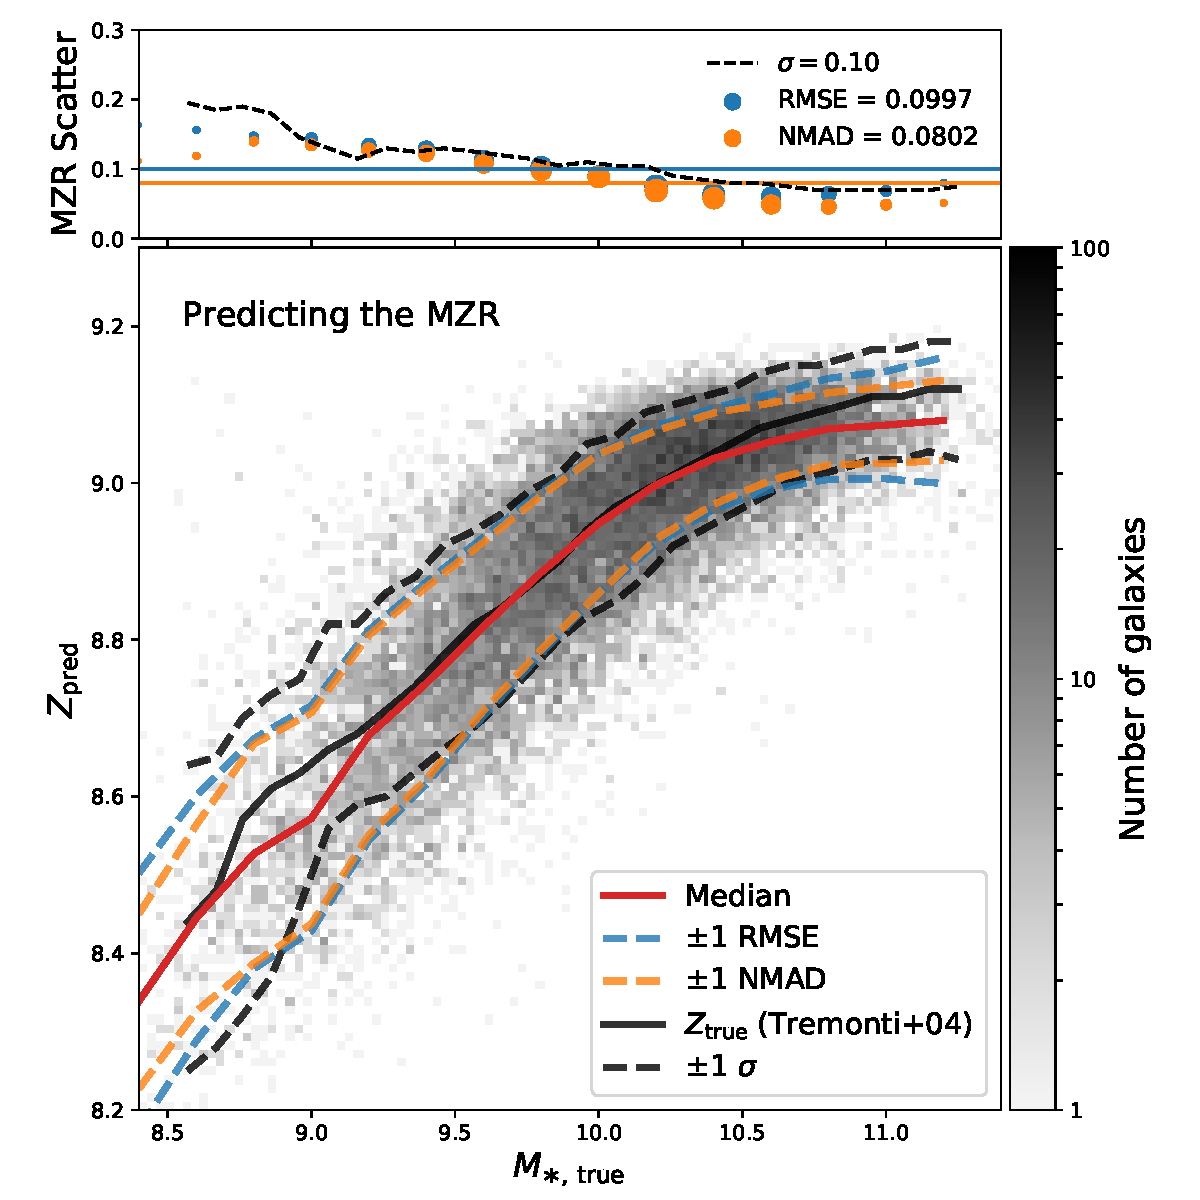
\includegraphics[width=\columnwidth]{05-mzr.pdf}
	\caption{\label{fig:mzr}
		In the main panel, the predicted MZR comparing true $M_\ast$ against CNN predicted $Z_{\rm pred}$ is shown in grayscale.
		The running median (solid red) and scatter (dashed blue and orange) are shown in 0.2~dex mass bins.
		For comparison, we also show the \citet{2004ApJ...613..898T} observed median and scatter binned by 0.1~dex in mass (solid and dashed black lines, respectively).
		In the panel above the main figure, we show the scatter in the predicted and empirical MZR.
		The standard deviation of the scatter in the MZR is shown as a dashed black line, while the blue and orange circles show the RMSE and NMAD, respectively, in bins of true $M_{\ast}$ (and whose marker sizes are proportional to the number of galaxies in the mass bin).
		Global scatter in the predicted MZR appears to be comparable or even lower than scatter from the true MZR.
	}
\end{figure}

In Figure~\ref{fig:mzr}, we show true stellar mass ($M_{\ast, \rm~true}$) against CNN-predicted metallicity.
For comparison, we also overlay the \cite{2004ApJ...613..898T} MZR and its scatter ($\sigma = 0.10$~dex).
The empirical median relations matches our predicted MZR median, and the lines marking different measures of scatter appear to match each other as well.
For $9.5 \leq \log (M_{\ast, true}/M_\odot) \leq 10.5$, the RMSE scatter in $Z_{\rm pred}$, shown in dashed blue, appears to be even tighter than the measured $\pm 1~\sigma$ (dashed black).
The same is true for the NMAD, which is even lower over the same interval.

In the upper panel of Figure~\ref{fig:mzr}, we present the scatter in both predicted and \cite{2004ApJ...613..898T} MZR binned by mass, which confirms that our CNN predicts a MZR that is at most equal (and possibly smaller) in scatter than one constructed using the true metallicity.
The mass bins for which predicted RMSE is lower than measured $\sigma$ are the ones which contain the most training examples.
Thus, it may be possible that if our data set was augmented to include additional low- and high-$M_{\rm \ast,true}$ galaxies, then the predicted RMSE (and NMAD) would be even lower.

The fact that a CNN trained on only $gri$ imaging is able to predict metallicity accurately enough to reproduce the MZR in terms of median and scatter is not trivial.
The error budget is very small: $\sigma = 0.10$~dex affords only, e.g., 0.05~dex of scatter when SFR is a controlled parameter plus 0.03~dex systematic scatter in $Z_{\rm true}$ measurements leaves only $\sim 0.08$~dex remaining for CNN systematics.
This is somewhat compatible with our result of RMSE($\Delta Z$) $= 0.085$.
However, this cannot be correct since it assumes that the CNN is recovering the FMR perfectly -- and as we have discussed before, it is highly unlikely that the CNN is sensitive to the SFR and therefore cannot probe the MZR at individual values of the SFR.
\textbf{The error budget for the MZR is already exceeded, too, as we have found RMSE = 0.10~dex for both the $Z_{\rm pred}-M_{\ast,\rm true}$ relation and the empirical MZR ($Z_{\rm true}-M_{\ast,\rm true}$) without accounting for the fact that $Z_{\rm pred}$ and $Z_{\rm true}$ differ by RMSE = 0.085~dex!
We thus find more evidence that the CNN has learned something from the SDSS $gri$ imaging that is different from, but at least as powerful as, the MZR.}

%NOTE: if we use gri imaging + SFR derived from spectroscopy, can we beat even the FMR?


%Note that we did not plot $M_{\rm \ast,~pred}$ because any possible covariance in the predicted metallicity and stellar mass would make such a MZR appear to be more correlated than it truly is.


%If there existed a fourth parameter, perhaps morphological in nature, then the marginalized MMR or FMR over particular values of this fourth parameter should be an even tighter relationship.
%Such a result would be analogous to how the MMR at any given star formation rate (SFR) has smaller scatter than over all SFRs.
%
%We find that the MMR constructed using SDSS-measured metallicity (via $R_{23}$) and the MMR constructed using CNN-predicted metallicity (from \textit{gri} imaging) are quantitatively different.
%In both cases we have used the GalSpecExtra catalog for stellar masses.
%The MMR using CNN metallicity has smaller scatter, where the weighted average ratio of scatter is NMAD(CNN)/NMAD(SDSS)~$= 0.821 \pm 0.077$.


%We also produced plots of the MMR using SDSS- and CNN-predicted masses, and SDSS metallicity from the GalSpecExtra catalog.
%Here the scatter in metallicity at given mass is again lower when using CNN predictions than for SDSS measurements.
%The scatter is smaller by a factor NMAD(CNN)/NMAD(SDSS)~ $= 0.811 \pm 0.057$.
%
%It is possible that the metallicity depends on some morphological component in addition to the emission lines informing the spectroscopic measurement.
%However, we believe that the qualitatively accurate MMR is actually artifact of the CNN's limitations rather than its strengths.
%Instead of finding a more fundamental representation of metallicity, the CNN likely detects the stellar mass.
%In the case of using our CNN to predict metallicity, the slope of the MMR is shallower than from the ``true'' data. 
%However, when the CNN is used to predict mass, the slope of is too steep.
%This effect is driven by the fact that the CNN is unable to predict the full range of metallicities or masses, since the fraction of training examples at extremely low or high values is small.
%\textbf{Therefore, the scatter in all of its predictions is narrower, such that when it predicts metallicity, the truncated range forces the MMR relationship to appear shallower, and when the CNN predicts $M_*$, the limited range in mass cause the MMR relationship to appear steeper.}
%
%Why then does the MMR hold at all?
%For if the CNN predicts, e.g., too narrow a distribution of metallicity, then what prevents those predictions from scattering over the full range in stellar mass?
%The answer is quite possibly that the CNN only ``sees'' the metallicity via the stellar mass, such that the predicted MMR is effectively a relationship between the predicted mass and the true mass.
%This theory is bolstered marginally by the fact that the fraction scatter for predicting mass is lower than for predicting metallicity (albeit not significantly so).
%More intuitively, we might believe that the CNN can ``see'' that read and dead elliptical galaxies are higher in stellar mass, and that blue irregulars are lower in stellar mass.
%Then the CNN simply needs to propagate the mass prediction through the tight $\sim 0.1$~dex MMR.
%
%\textbf{How then can we achieve a NMAD~=~0.067~dex in metallicity by noisily propagating a signal with NMAD~=~0.22 scatter through the MMR which has 0.1~dex intrinsic scatter (Tremonti et al. 2004)?}
%
%M/L ratio of redder galaxies are higher at fixed luminosity (Bell \& de Jong 2001; Kauffman+03).





%\subsection{Can stellar population age explain some of the scatter in the FMR?}

%\subsection{Why do CNNs work so well at predicting spectroscopic quantities?}
%Can we find a non-CNN parameter or method of explaining the scatter?

\section{Future Applications}\label{sec:future}

An future extension to our work might be to repeat our analysis but to instead train on simulated data.
Another is to feed SFR to the CNN and see if we can beat the FMR.

\section{Summary}\label{sec:summary}



Lorem ipsum dolor sit amet, consectetur adipisicing elit, sed do eiusmod tempor incididunt ut labore et dolore magna aliqua. Ut enim ad minim veniam, quis nostrud exercitation ullamco laboris nisi ut aliquip ex ea commodo consequat. Duis aute irure dolor in reprehenderit in voluptate velit esse cillum dolore eu fugiat nulla pariatur. Excepteur sint occaecat cupidatat non proident, sunt in culpa qui officia deserunt mollit anim id est laborum.

Our main conclusions are the following:
\begin{enumerate}
	\item Lorem ipsum dolor sit amet, consectetur adipisicing elit, sed do eiusmod tempor incididunt ut labore et dolore magna aliqua. Ut enim ad minim veniam, quis nostrud exercitation ullamco laboris nisi ut aliquip ex ea commodo consequat. Duis aute irure dolor in reprehenderit in voluptate velit esse cillum dolore eu fugiat nulla pariatur. Excepteur sint occaecat cupidatat non proident, sunt in culpa qui officia deserunt mollit anim id est laborum.

	\item Lorem ipsum dolor sit amet, consectetur adipisicing elit, sed do eiusmod tempor incididunt ut labore et dolore magna aliqua. Ut enim ad minim veniam, quis nostrud exercitation ullamco laboris nisi ut aliquip ex ea commodo consequat. Duis aute irure dolor in reprehenderit in voluptate velit esse cillum dolore eu fugiat nulla pariatur. Excepteur sint occaecat cupidatat non proident, sunt in culpa qui officia deserunt mollit anim id est laborum.
\end{enumerate}

\section*{Acknowledgements}
\editorial{The authors also wish to thank the anonymous referee whose comments and suggestions significantly improved both the quality and clarity of this work.}
The authors also thank David Shih and Matthew Buckley for use of their GPU cluster at Rutgers University High Energy Experimental Physics department. %, and Kartheik Iyer for providing SED fits as benchmark as well as for valuable discussion.
This research made use of the {\sc IPython} package \citep{Perez2007} and {\sc matplotlib}, a Python library for publication quality graphics \citep{Hunter2007}. Funding for the SDSS and SDSS-II has been provided by the Alfred P. Sloan Foundation, the Participating Institutions, the National Science Foundation, the U.S. Department of Energy, the National Aeronautics and Space Administration, the Japanese Monbukagakusho, the Max Planck Society, and the Higher Education Funding Council for England. The SDSS Web Site is \url{http://www.sdss.org/}.

%%%%%%%%%%%%%%%%%%%% REFERENCES %%%%%%%%%%%%%%%%%%
% The best way to enter references is to use BibTeX:
\bibliographystyle{mnras}
\bibliography{bibliography} % if your bibtex file is called example.bib

%%%%%%%%%%%%%%%%% APPENDICES %%%%%%%%%%%%%%%%%%%%%
\appendix
%
\section{Residual convolutional neural networks}
%
% If you want to present additional material which would interrupt the flow of the main paper,
% it can be placed in an Appendix which appears after the list of references.



We find that a 34-layer resnet (Resnet-34) architecture can be trained efficiently on a Pascal P100 with 16~GB of memory.
Using the hyperparameters described below, an epoch takes about 60~seconds to train.
We initialize our resnet with pretrained weights from the ImageNet (Russakovsky et al. 2014; He et al. 2015) 1.7~million image data set trained to recognize 1000 classes of objects found on Earth (i.e., cats, dogs, or cars).
In practice, the filters learned through the early layers of the pretrained CNN can be used for other image recognition tasks, aptly named ``transfer learning'' (cite).


\subsection{Hyperparameter selection}

\subsection{Data augmentation}
Nearly all neural networks benefit from larger training samples because they help prevent overfitting.
Outside of the local Universe, galaxies are seen at nearly random orientation; such invariance permits synthetic data to be generated from rotations and flips of the training images.
Each image is fed into the network along with four augmented versions, thus increasing the total training sample by a factor of five.
%Additional small zooms of $< 5\%$ may also be applied to enlarge the training size.
This technique is called data augmentation, and is particularly helpful for the network to learn uncommon or unrepresented truth values (e.g., in our case, very metal-poor or metal-rich galaxies).
Each training-augmentation is fed-forward through the network and gradient contributions are computed together as part of the same mini-batch.
A similar process is applied to the network during predictions, which is called test-time augmentation (TTA).
Synthetic images are generated according to the same rules applied to the training data set. 
The CNN predicts an ensemble average over the augmented images.
It has been found that data augmentation improves predictions by as much as $\sim 20\%$ (cite).

\subsection{Cyclical learning rate annealing}
The learning rate determines how large of a step each network weight takes in the direction of the backpropagated error.
A large learning rate thus forces the weights to make large updates, which generally prevents overfitting but also may cause the parameters to overshoot minima in the loss function landscape.
A small learning rate may allow the weights to get stuck in a local minima near their initial positions, or also might cause the network to learn very slowly.
The number of local minima increases exponentially with dimensionality (cite), so selecting a low learning rate does not ensure that the network will eventually make it to near the global minimum.
Therefore, it is often useful to anneal, or reduce, the learning rate from a high value in the beginning -- which allows the weights to find the right ballpark values -- to a low value -- which allows the weights to take finer steps near the global minimum -- over the course of multiple training epochs.

In practice, annealing can be enforced manually, e.g., the learning rate might be reduced by a factor of 10 every time the loss function plateaus over a number of epochs.
Eventually even reduced learning rates do not permit additional improvement of the loss, and so the training period is concluded.
We instead use a method called cosine annealing, during which the learning rate is annealed continuously over one or more epochs for \textit{each} mini-batch until it eventually reaches zero.


We employ stochastic gradient descent with restarts (SGDR), over progressively longer training cycles, and restart cosine annealing over each cycle (Leslie Smith 2015?). 
For example, the first cycle comprises one epoch during which the learning rate is cosine annealed.
It then trains for another cycle with cosine annealing, which starts at the same learning rate but is annealed over twice the duration (two epochs).
These ``restarts'' have been shown to kick the weights configuration out of saddle points in the loss of some high-dimensional parameter space.
Training can then proceed past what appear to be local minima but are actually saddle points (where gradient descent generally performs poorly).


\subsection{Layer learning rates}
ADD MORE HERE

Frozen training to get final activates in right ``ballpark.''
We then unfreeze all layers and train using different rates in different layer groups.

\subsection{Batch normalization and Dropout}

Batch normalization (BN; 1502.03167) is a technique developed to fix the vanishing gradients problem which make deep networks inefficiently slow to train.
The issue arises when gradients are backpropagated through deep neural networks to update weights, and loss contributions become vanishingly small except only when the weights have small magnitudes.
Normalizing the inputs to each mini-batch mean and standard deviation somewhat remedies the problem, and has been applied to (convolutional) neural networks since the 1990s.
BN extends this normalization to all activations in hidden layers, thus adding two hyperparameters which modulate the mean and standard deviation of each layer to zero and unity, respectively.
The BN hyperparameters are learned for each mini-batch and are updated in addition to weight parameters during the backward pass.
% if confused refer to  https://kratzert.github.io/2016/02/12/understanding-the-gradient-flow-through-the-batch-normalization-layer.html4

Without BN, activations in any given layer may span a large range and contributions from certain parts of the network may become dwarfed by others.
After the normalization step, all pre-activations are on the same scale and thus gradient descent steps can more efficiently traverse the loss function space.
Training proceeds more rapidly and converges toward a solution more quickly.
Choice of mini-batch size also impacts the learning rate, as small batch size increases stochasticity in each gradient.
Large batch size allows for better parallelization on the GPU and ensures smoother gradients.
We note that smooth gradients across mini-batches can prevent the solution from hopping out of local basins, and negatively impact performance.
Increasing the learning rate as batch size is increased can resolve this problem, at least in part, but limits the convergence ability of the network (until the rate is annealed).
We find in practice that batch sizes between 128 and 512 work best at balancing noisy gradients and learning rate.


Dropout is a method of disabling a random subset of connections after linear layers for each mini-batch (Hinton et al. 2012).
By removing random connections between fully-connected layers, dropout effectively treats each mini-batch as one in an ensemble of random training subsets .
It is instructive to think of each mini-batch in the full training data as analogous to a decision tree in a random forest.
The ensemble of learned gradients is less prone to overfit the training data set because the network is forced to discard random (and potentially valuable) information.
The resulting network is better able to, for example, learn subtle differences in the data that would otherwise be ignored when more obvious features dominate the gradient descent process.
Since our Resnet architecture is broadly separated into multiple groups of layers, we can apply lower dropout rate at earlier layers in order to ensure that those filters are learned more quickly.
Using a differential dropout rate is sensible because filters learned in the first few layers of the network tend to be Gabor filters and edges in general, and there is little risk of overfitting when such low-level abstractions are always necessary for learning high-level features in the middle and final layers.

During validation and testing, dropout is not used because all of the data is useful for predictive power.
We use dropout rates of 0.25 for the linear layer after the early group, and 0.50 at the later linear layer.
We find that dropout combined with BN -- although not recommended in the original paper -- work in tandem to boost training speeds and avoid overfitting.



% Don't change these lines
\bsp	% typesetting comment
\label{lastpage}
\end{document}
